\Transcb{yellow}{blue}{Possible high-energy sources}
\twocolumn
\begin{center}
{\blue Active Galactic Nuclei (AGN)}\\[1cm]
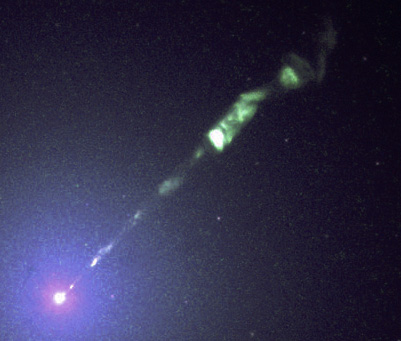
\includegraphics[keepaspectratio,width=13cm]{M87jet}
\end{center}

\newpage

\begin{center}
{\blue Gamma Ray Bursts (GRBs)}\\[1cm]
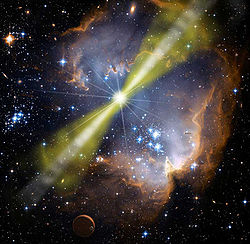
\includegraphics[keepaspectratio,width=6cm]{grb}\\[3mm]
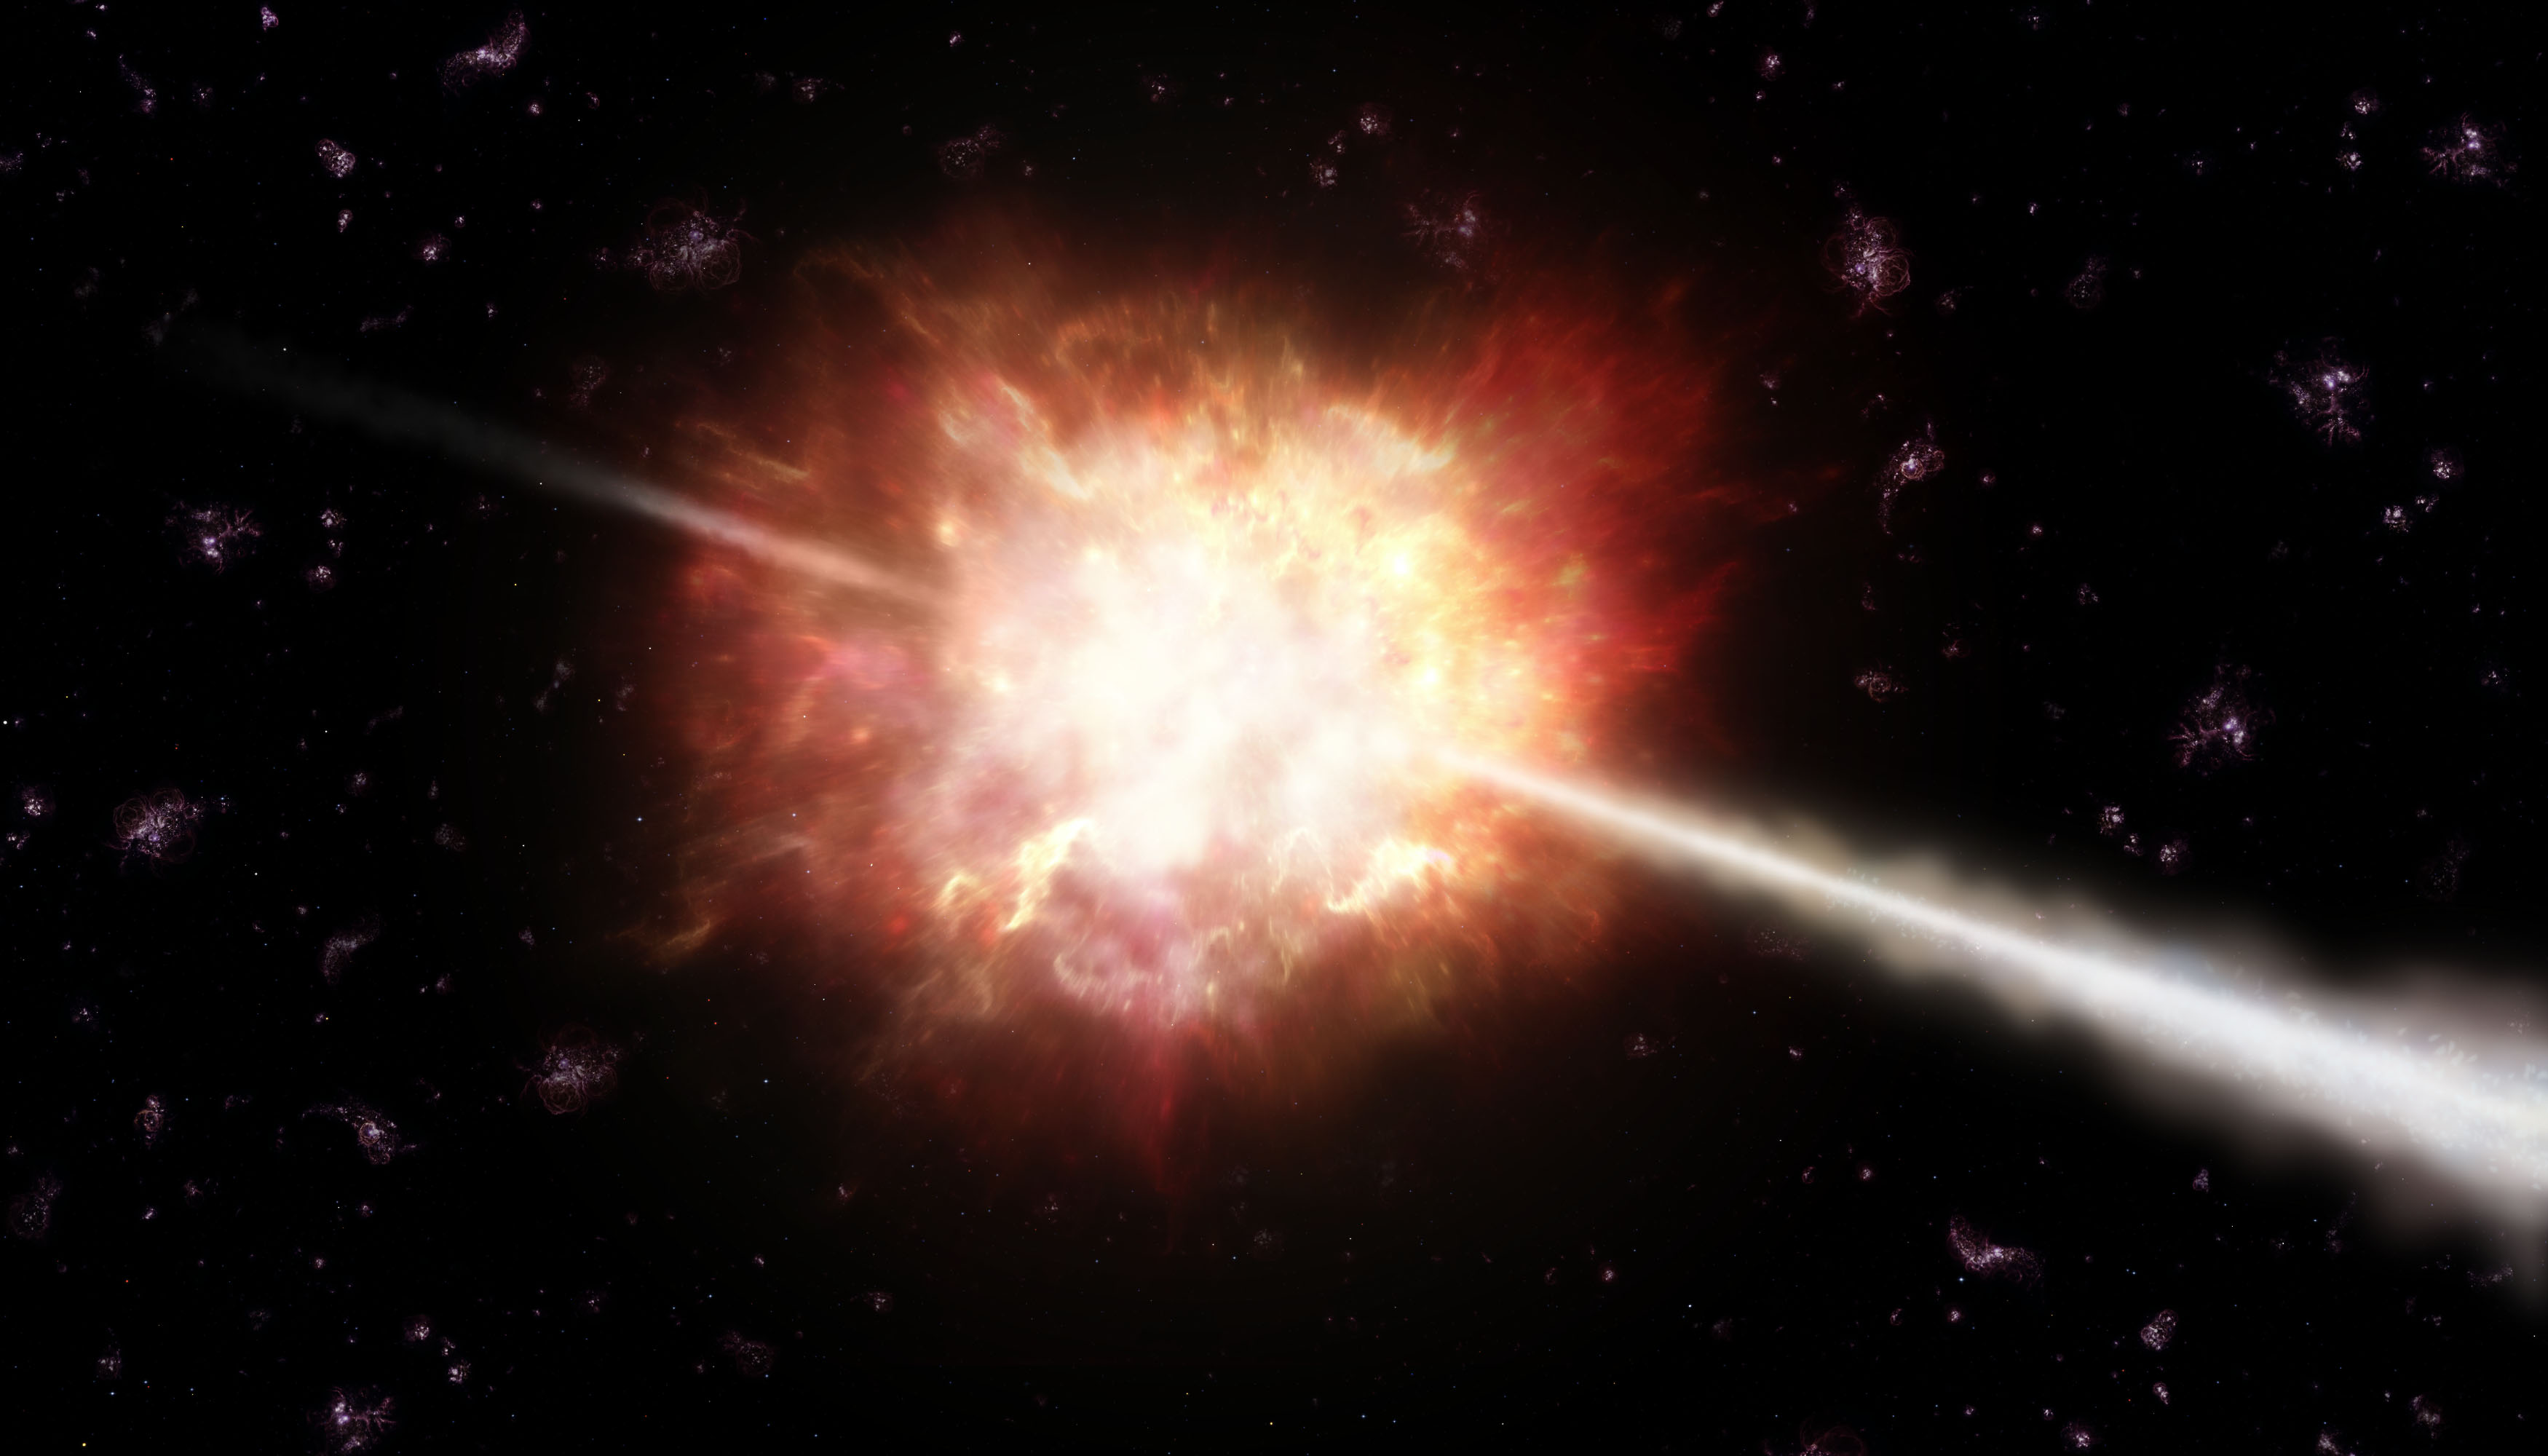
\includegraphics[keepaspectratio,width=12cm]{grb2}
\end{center}

\Tr
\begin{dinglist}{228}
\item Engines which power AGN
\begin{itemize}
\item Acceleration via shock waves in the jets
\item Jet directed to us $\rightarrow$ Blazar
\item[] Markarian 421 and 501
\end{itemize}
\item Gamma Ray Bursts
\begin{itemize}
\item 'Hypernovae' $\rightarrow$ Black hole
\item NS+NS or NS+BH mergers
\item[] {\blue Also shock wave acceleration}
\end{itemize}
\item Cold dark matter (WIMPs, SUSY particles)
\begin{itemize}
\item Annihilation $\rightarrow$ {\blue High $E$ neutrinos}
\item[] {\red WIMPs at the center of Sun, Earth ?}
\end{itemize}
\item[$\ast$] \colorbox{yellow}{Most extreme events are GRBs}
\item[] {\blue Can GRBs produce the flux at the ankle ?}
\item[] Waxman\&Bahcall PRL 78 (1997) 2292
\end{dinglist}

\newpage

\begin{center}
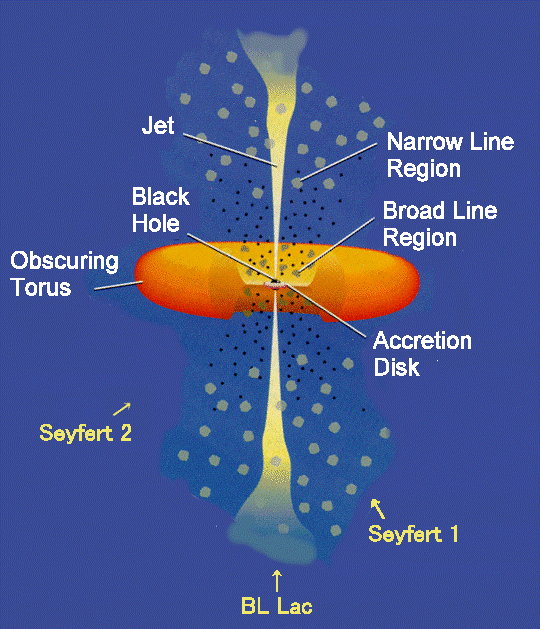
\includegraphics[keepaspectratio,width=13cm]{agn-1}
\end{center}

\Tr
\begin{center}
{\blue Processes in the jet}\\[5mm]
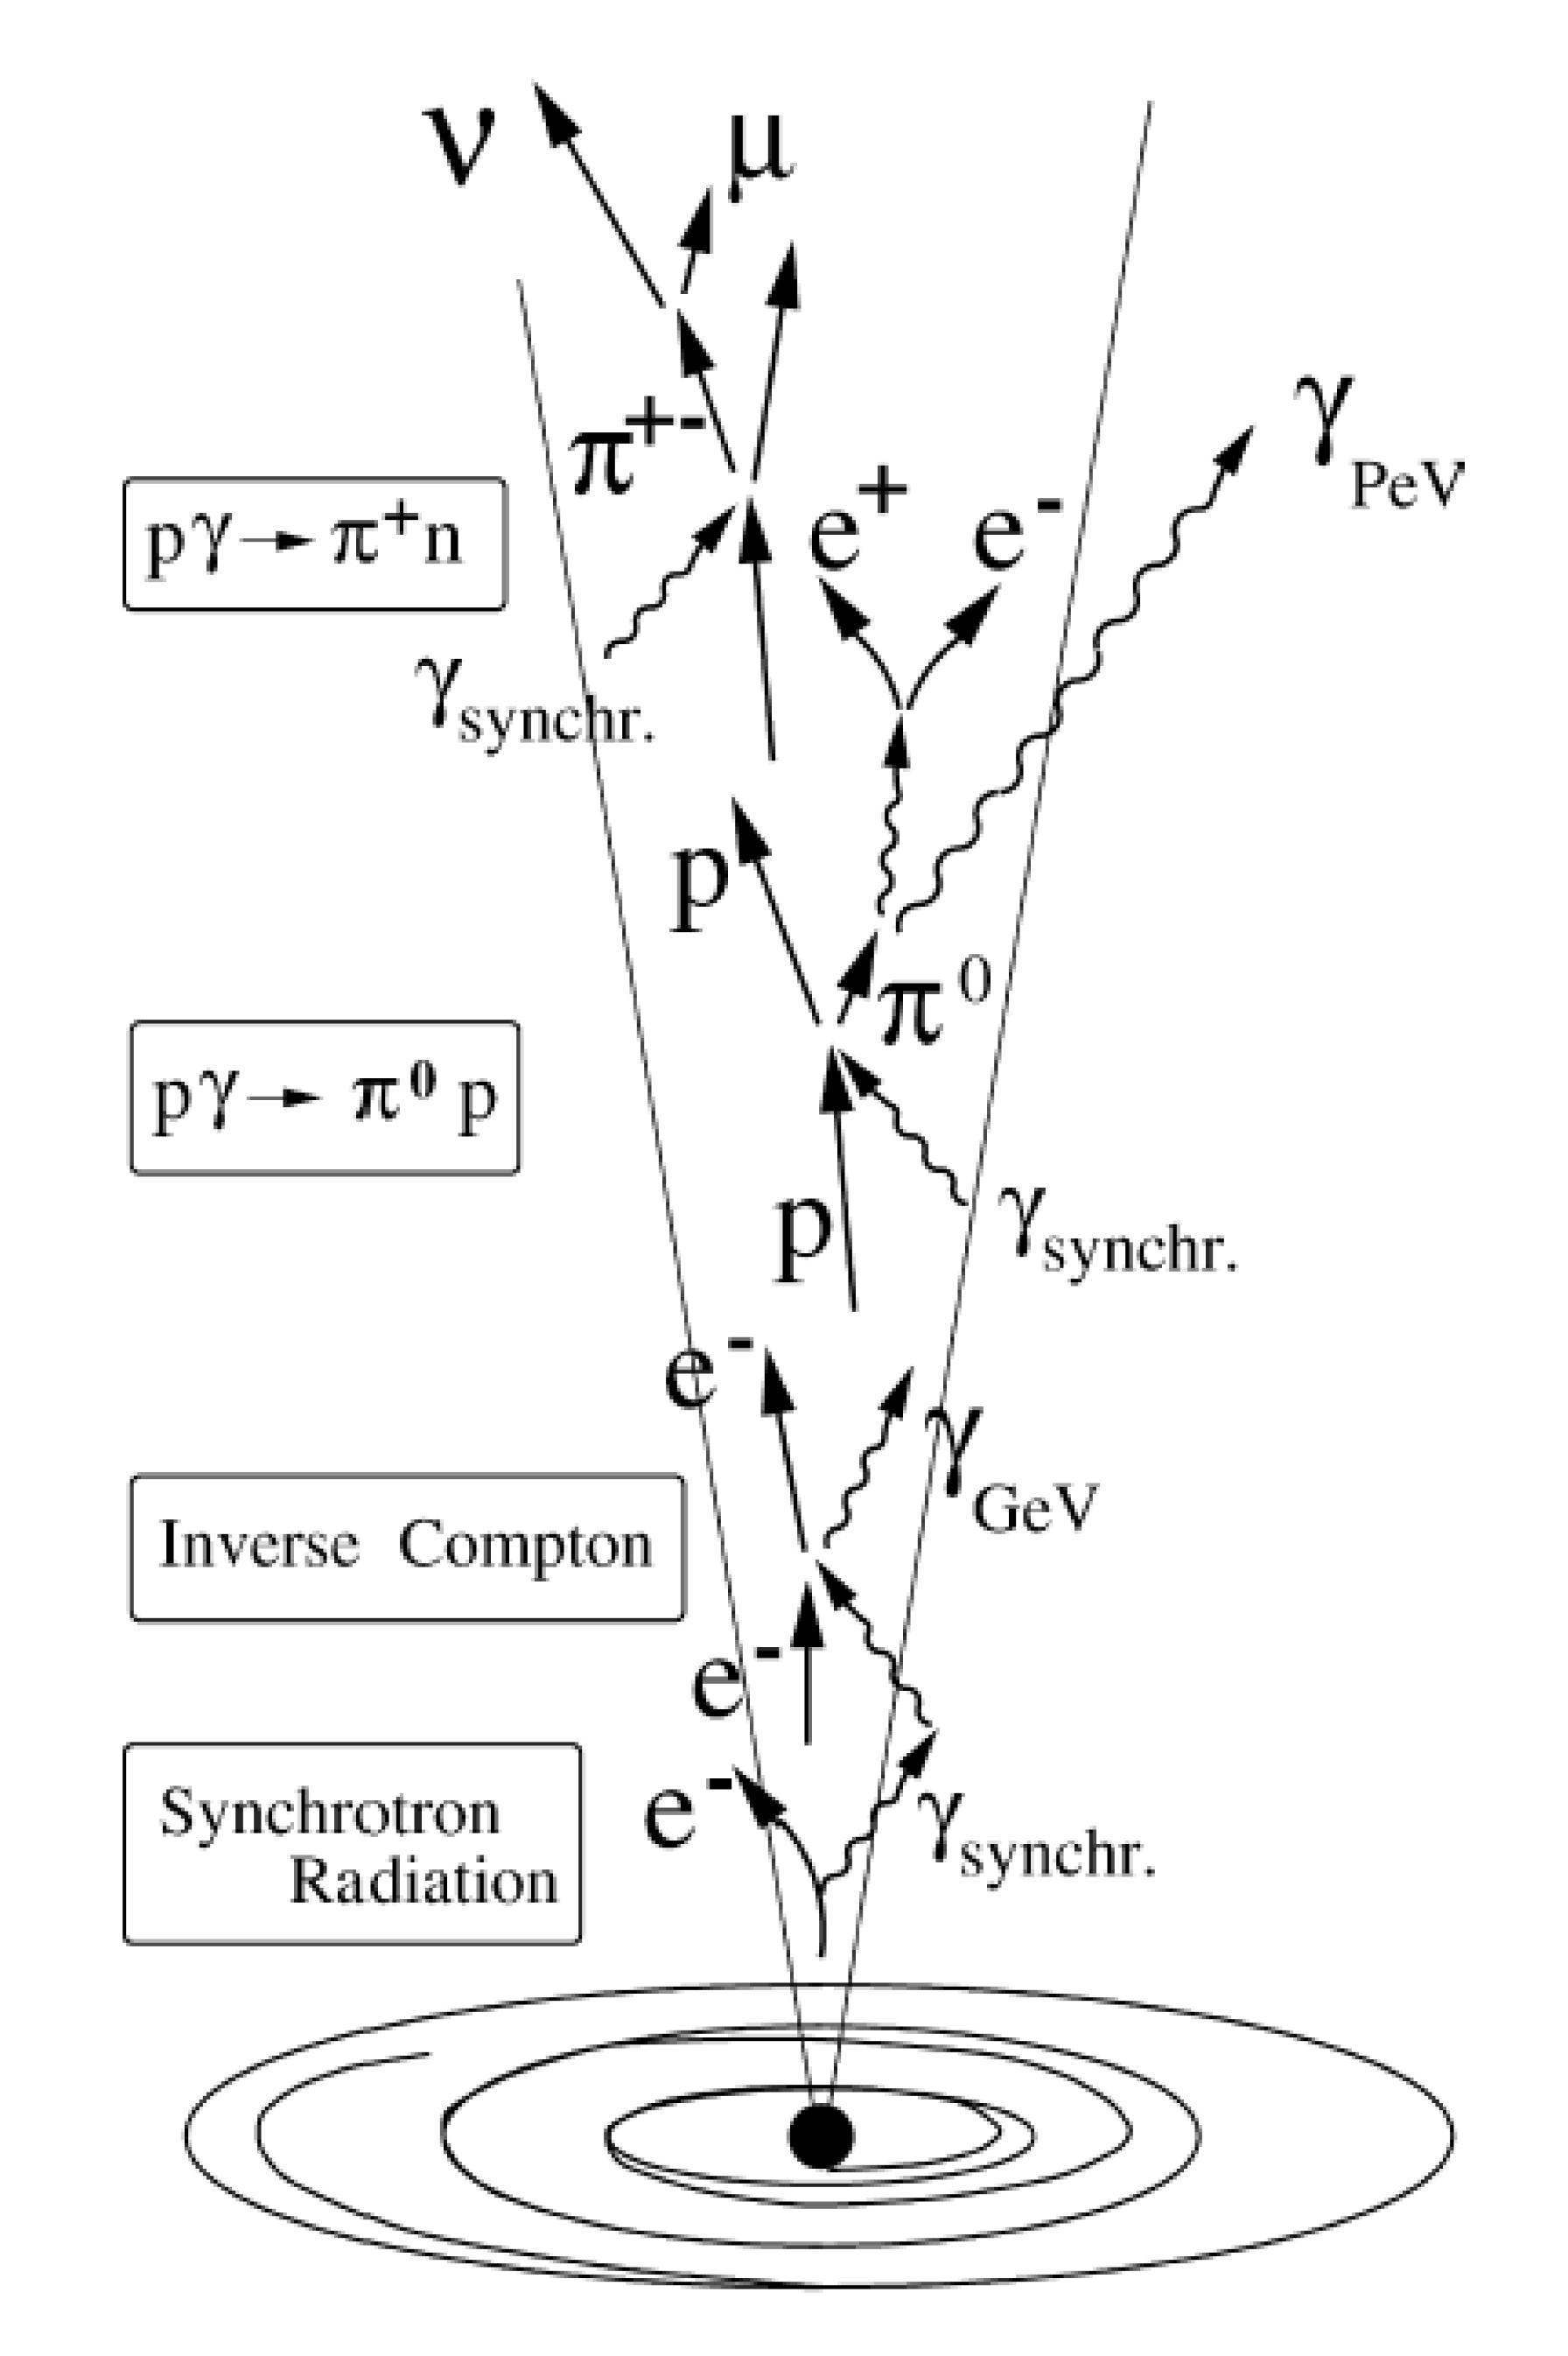
\includegraphics[keepaspectratio,height=12cm]{jet}
\end{center}
%
\colorbox{yellow}{Can this GRB fireball model be probed ?}

\newpage

\begin{center}
{\blue Neutrino production mechanism}\\[5mm]
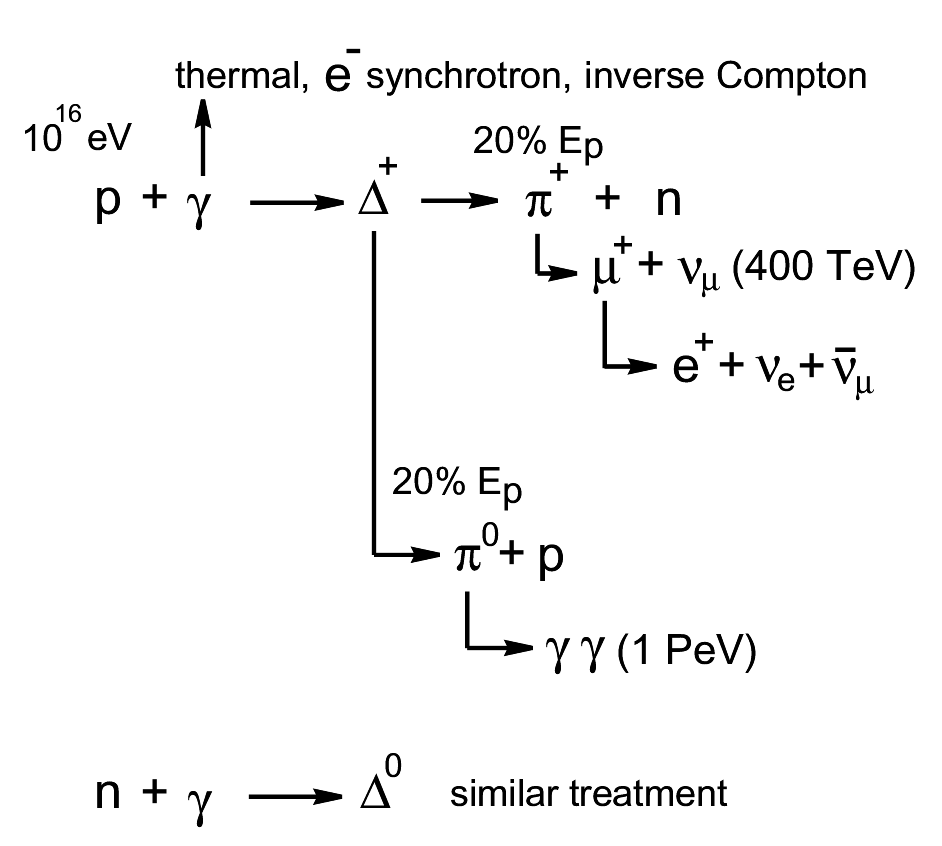
\includegraphics[keepaspectratio,width=12cm]{grb-engine2}
\end{center}
%
$\Delta$ production threshold~: $E_{\gamma} \ge 10$ eV\\
(UV photons)
